\documentclass{article}
\usepackage{graphicx} % Extended graphics inclusions
\usepackage{float}
\usepackage{url} % For \url{}
\usepackage{../config/atxy} % For front cover
\usepackage{amsfonts} % Needed for some fonts
\usepackage[usenames]{color} % Needed for colored R input/output
\usepackage{pdfcolmk} % Correct some problems with the color stack


\title{Installation of a local ACNUC socket server and of a local ACNUC database on your machine.}
\author{Penel, S.}

\usepackage{/Library/Frameworks/R.framework/Resources/share/texmf/Sweave}
\begin{document}
%
% To change the R input/output style:
%
\definecolor{Soutput}{rgb}{0,0,0.56}
\definecolor{Sinput}{rgb}{0.56,0,0}
\DefineVerbatimEnvironment{Sinput}{Verbatim}
{formatcom={\color{Sinput}},fontsize=\footnotesize, baselinestretch=0.75}
\DefineVerbatimEnvironment{Soutput}{Verbatim}
{formatcom={\color{Soutput}},fontsize=\footnotesize, baselinestretch=0.75}
%
% This removes the extra spacing after code and output chunks in Sweave,
% but keeps the spacing around the whole block.
%
\fvset{listparameters={\setlength{\topsep}{0pt}}}
\renewenvironment{Schunk}{\vspace{\topsep}}{\vspace{\topsep}}
%
% Rlogo
%
\newcommand{\Rlogo}{\protect
\includegraphics[height=1.8ex,keepaspectratio]{../figs/Rlogo.pdf}}
%
% Shortcut for seqinR:
%
\newcommand{\seqinr}{\texttt{seqin\bf{R}}}
\newcommand{\Seqinr}{\texttt{Seqin\bf{R}}}
\fvset{fontsize= \scriptsize}
%
% R output options and libraries to be loaded.
%
%
%  Sweave Options
%
% Put all figures in the fig folder and start the name with current file name.
% Do not produce EPS files
%


\maketitle
\tableofcontents
% BEGIN - DO NOT REMOVE THIS LINE



%%%%%%%%%%%%%%%%%%%%%%%
\section{Introduction}
%%%%%%%%%%%%%%%%%%%%%%%

This chapter is under development.

%%%%%%%%%%%%%%%%%%%%%%%%%%%%
\section{System requirement}
%%%%%%%%%%%%%%%%%%%%%%%%%%%%

Basically if you are installing \Rlogo{} from the
sources, you should be able to build a ACNUC socket server.
The socket server will build under a number of common Unix and Unix-alike
platforms. You will need several tools: programs are written in C thus 
you will need a
means of compiling C (as gcc compilation tools for linux or unix, Apple
Developer Tools  for MacOSX). You need as well library zlib and sockets
(standards on linux and unix).


%%%%%%%%%%%%%%%%%%%%%%%%%%%%%%%%%%%%%%%%%%%%%%%%%%%%%%%%%%%%%%
\section{Setting a local ACNUC database to be queried by the server}
%%%%%%%%%%%%%%%%%%%%%%%%%%%%%%%%%%%%%%%%%%%%%%%%%%%%%%%%%%%%%%

First of all yo need an ACNUC database, built by yourself or  downloaded from the PBIL ftp server.
An ACNUC database is composed of two sets of files:
\begin{enumerate}
	\item  the acnuc index files.
	\item  the database files (\textit{i.e.} flat files in EMBL/GenBank or SwissProt format).
\end{enumerate}

These two sets will be located  in the \texttt{index} and  \texttt{flat\_files} directories  respectively.

An example of an ACNUC database is available on the PBIL ftp server  at this url:
\url{ftp://pbil.univ-lyon1.fr/pub/seqinr/demoacnuc/acnucdatabase.tar.Z}.
 
You may install the database as it follows:
Let \texttt{ACNUC\_HOME} be the base directory for ACNUC installation.

\begin{Schunk}
\begin{Sinput}
 dir.create("./ACNUC_HOME", showWarning = FALSE)
\end{Sinput}
\end{Schunk}


Let ACNUC\_HOME/ACNUC\_DB be the  directory where you want to install the databases and ACNUC\_HOME/ACNUC\_DB/demoacnuc 
the directory where you want to install the demo database.

\begin{Schunk}
\begin{Sinput}
 dir.create("./ACNUC_HOME/ACNUC_DB", showWarning = FALSE)
 dir.create("./ACNUC_HOME/ACNUC_DB/demoacnuc", showWarning = FALSE)
\end{Sinput}
\end{Schunk}


\begin{itemize}
\item Dowload the ACNUC database in the ./ACNUC\_HOME/ACNUC\_DB/demoacnuc/ directory.

% Mettre eval=F apres premier download
\begin{Schunk}
\begin{Sinput}
 download.file("ftp://pbil.univ-lyon1.fr/pub/seqinr/demoacnuc/acnucdatabase.tar.Z", 
     destfile = "./ACNUC_HOME/ACNUC_DB/demoacnuc/acnucdatabase.tar.Z")
\end{Sinput}
\end{Schunk}


\item Uncompress and untar the \texttt{acnucdatabase.tar.Z} file 

\begin{Schunk}
\begin{Sinput}
 pwd <- getwd()
 setwd("./ACNUC_HOME/ACNUC_DB/demoacnuc/")
 system("gunzip -f acnucdatabase.tar.Z")
 system("tar -xvf acnucdatabase.tar")
 system("rm -f acnucdatabase.tar")
 setwd(pwd)
\end{Sinput}
\end{Schunk}

\end{itemize}
Now you sould get the following directories:
\begin{verbatim}
ACNUC_HOME/ACNUC_DB/demoacnuc/index
ACNUC_HOME/ACNUC_DB/demoacnuc/flat_files
\end{verbatim}

The directory \texttt{ACNUC\_HOME/ACNUC\_DB/demoacnuc} contains: 
\begin{Schunk}
\begin{Sinput}
 dir("./ACNUC_HOME/ACNUC_DB/demoacnuc")
\end{Sinput}
\begin{Soutput}
[1] "flat_files" "index"     
\end{Soutput}
\end{Schunk}

These directories contain respectively:

\begin{Schunk}
\begin{Sinput}
 dir("./ACNUC_HOME/ACNUC_DB/demoacnuc/index")
\end{Sinput}
\begin{Soutput}
 [1] "ACCESS"                  "AUTHOR"                 
 [3] "BIBLIO"                  "EXTRACT"                
 [5] "HELP"                    "HELP_WIN"               
 [7] "KEYWORDS"                "LOCUS"                  
 [9] "LONGL"                   "MERES"                  
[11] "SHORTL"                  "SMJYT"                  
[13] "SPECIES"                 "SUBSEQ"                 
[15] "TAXIDS"                  "TEXT"                   
[17] "custom_qualifier_policy"
\end{Soutput}
\begin{Sinput}
 dir("./ACNUC_HOME/ACNUC_DB/demoacnuc/flat_files")
\end{Sinput}
\begin{Soutput}
[1] "escherichia.dat" "id.log"          "yeast.dat"      
\end{Soutput}
\end{Schunk}


This database contains the complete genome of \textit{Escherichia coli} 
K12 W3110 and \textit{Saccharomyces cerevesiae}.

%%%%%%%%%%%%%%%%%%%%%%%%%%%%%%%%%%%%%%%%%%%%%%%%%%%%%%%%%%
\section{Build the ACNUC sockets server from the sources.}
%%%%%%%%%%%%%%%%%%%%%%%%%%%%%%%%%%%%%%%%%%%%%%%%%%%%%%%%%%

Once you have a local  ACNUC database available on your server you need to install the sockets server.

\subsection{Download the sources.}
%%%%%%%%%%%%%%%%%%%%%%%%%%%%%%%%%%

The code source of the racnucd server is available on the PBIL server  at this url:
\begin{verbatim}
http://pbil.univ-lyon1.fr/databases/acnuc/racnucd.html
\end{verbatim}
Alternatively you can download directly  the source from the ftp at:
\begin{verbatim}
ftp://pbil.univ-lyon1.fr/pub/acnuc/unix/racnucd.tar
\end{verbatim}

\subsection{Build the ACNUC sockets server.}
%%%%%%%%%%%%%%%%%%%%%%%%%%%%%%%%%%%%%%%%%%%%

You may install the racnucd server as it follows:
let ACNUC\_HOME/ACNUC\_SOFT/ be the base directory for the ACNUC softs.

\begin{Schunk}
\begin{Sinput}
 dir.create("./ACNUC_HOME/ACNUC_SOFT", showWarning = FALSE)
\end{Sinput}
\end{Schunk}

\begin{itemize}
\item Dowload the \texttt{racnucd.tar} file into ACNUC\_HOME/ACNUC\_SOFT.

% Mettre eval=F apres premier download
\begin{Schunk}
\begin{Sinput}
 download.file("ftp://pbil.univ-lyon1.fr/pub/acnuc/unix/racnucd.tar", 
     destfile = "./ACNUC_HOME/ACNUC_SOFT/racnucd.tar")
\end{Sinput}
\end{Schunk}

\item Untar the \texttt{racnucd.tar} file 

\begin{Schunk}
\begin{Sinput}
 setwd("./ACNUC_HOME/ACNUC_SOFT/")
 system("tar -xvf racnucd.tar")
 system("rm -f racnucd.tar")
 setwd(pwd)
\end{Sinput}
\end{Schunk}

\end{itemize}
Now you sould get the following directory:


\begin{Schunk}
\begin{Sinput}
 dir("./ACNUC_HOME/ACNUC_SOFT/")
\end{Sinput}
\begin{Soutput}
[1] "racnucd"
\end{Soutput}
\begin{Sinput}
 dir("./ACNUC_HOME/ACNUC_SOFT/racnucd/")
\end{Sinput}
\begin{Soutput}
 [1] "bit.c"                "dbplaces"             "dir_acnuc.h"         
 [4] "dir_io.c"             "dir_io.h"             "execute.c"           
 [7] "execute.h"            "extract.c"            "knowndbs"            
[10] "lngbit.c"             "makefile"             "md5.c"               
[13] "misc_acnuc.c"         "ordre.h"              "parser.c"            
[16] "prep_acnuc_requete.c" "pretty_seq.c"         "proc_requete.c"      
[19] "racnucd.ini"          "requete_acnuc.h"      "serveur.c"           
[22] "serveur.h"            "simext.h"             "use_acnuc.c"         
[25] "utilquery.c"          "zsockw.c"            
\end{Soutput}
\end{Schunk}

Go into \texttt{ACNUC\_HOME/ACNUC\_SOFT/racnucd/} and type \texttt{make}.
This should create the \textbf{racnucd} executable.

\begin{Schunk}
\begin{Sinput}
 setwd("./ACNUC_HOME/ACNUC_SOFT/racnucd")
 system("make")
 dir(pattern = "racnucd")
\end{Sinput}
\begin{Soutput}
[1] "racnucd"     "racnucd.ini"
\end{Soutput}
\begin{Sinput}
 setwd(pwd)
\end{Sinput}
\end{Schunk}

\subsection{Setting the ACNUC sockets server.}
%%%%%%%%%%%%%%%%%%%%%%%%%%%%%%%%%%%%%%%%%%%%%%

The server is configured by several parameters described in a configuration file \textbf{racnuc.ini}.
The \textbf{racnucd.ini} file is structued as follows:


\begin{Schunk}
\begin{Sinput}
 cat(readLines("./ACNUC_HOME/ACNUC_SOFT/racnucd/racnucd.ini"), 
     sep = "\n")
\end{Sinput}
\begin{Soutput}
port=5558
maxtime=8000
known_db_file=knowndbs
db_env_names=dbplaces
\end{Soutput}
\end{Schunk}

\begin{itemize}
\item \textbf{port} is the port of the socket server 
\item \textbf{maxtimle} is the time delay of the connection
\item \textbf{knowndbs} is a file containing the list of available databases
\item \textbf{dbplaces} is a file containing the path of the available databases
\end{itemize}



You may want to change the port of the socket server, according to the availabilities and restricttions on your machine.
For example , lets use the port 49152 in a new racnucd.new file.

\begin{Schunk}
\begin{Sinput}
 initline <- readLines("./ACNUC_HOME/ACNUC_SOFT/racnucd/racnucd.ini")
 initline[1] = "port=49152"
 writeLines(initline, "./ACNUC_HOME/ACNUC_SOFT/racnucd/racnucd.new")
 cat(readLines("./ACNUC_HOME/ACNUC_SOFT/racnucd/racnucd.new"), 
     sep = "\n")
\end{Sinput}
\begin{Soutput}
port=49152
maxtime=8000
known_db_file=knowndbs
db_env_names=dbplaces
\end{Soutput}
\end{Schunk}

 
\subsubsection{Configuring the knowndbs file.}
%%%%%%%%%%%%%%%%%%%%%%%%%%%%%%%%%%%%%%%%%

The \textbf{knowndbs} contains:

\begin{Schunk}
\begin{Sinput}
 cat(readLines("./ACNUC_HOME/ACNUC_SOFT/racnucd/knowndbs"), 
     sep = "\n")
\end{Sinput}
\begin{Soutput}
embl | on |    | EMBL sequence data library | 
swissprot   | on |  | UniProt |
\end{Soutput}
\end{Schunk}

Each line defines a database,  the four fields indicating respectively the name
 of the database, its status  (\textit{on} or \textit{off}), a tag and a short description.
 
You should set the files \textbf{knowndbs}  according to your installation.
Let's call the database you installed previously \textit{demoacnuc}.
Modify  the \textbf{knowndbs} as follows:
\begin{verbatim}
demoacnuc | on |    | Demo Database | 
\end{verbatim}

\begin{Schunk}
\begin{Sinput}
 writeLines("demoacnuc | on |    | Demo Database | ", "./ACNUC_HOME/ACNUC_SOFT/racnucd/knowndbs")
 knowndbs <- readLines("./ACNUC_HOME/ACNUC_SOFT/racnucd/knowndbs")
 cat(knowndbs, sep = "\n")
\end{Sinput}
\begin{Soutput}
demoacnuc | on |    | Demo Database | 
\end{Soutput}
\end{Schunk}

\subsubsection{Configuring the dbplaces file.}
%%%%%%%%%%%%%%%%%%%%%%%%%%%%%%%%%%%%%%%%%%%%%%


The \textbf{dbplaces} contains:

\begin{Schunk}
\begin{Sinput}
 dbplaces <- readLines("./ACNUC_HOME/ACNUC_SOFT/racnucd/dbplaces")
 cat(dbplaces, sep = "\n")
\end{Sinput}
\begin{Soutput}
#defines location of acnuc databases index files and flat files

setenv 	swissprot 	'/Users/mgouy/Documents/acnuc/petite/swissprot /Users/mgouy/Documents/acnuc/petite/swissprot'
setenv 	embl 	'/Users/mgouy/Documents/acnuc/petite/embl /Users/mgouy/Documents/acnuc/petite/embl'
\end{Soutput}
\end{Schunk}

Each line set the acnuc and gcgacnuc variables for each   database.


You should set the files \textbf{dbplaces}  according to your installation:
 modify  the \textbf{dbplaces} as follows:
\begin{verbatim}
setenv  demoacnuc       'ACNUC_HOME/ACNUC_DB/demoacnuc/index ACNUC_HOME/ACNUC_DB/demoacnuc/flat_files'
\end{verbatim}

\begin{Schunk}
\begin{Sinput}
 indexpath <- normalizePath("./ACNUC_HOME/ACNUC_DB/demoacnuc/index")
 ffpath <- normalizePath("./ACNUC_HOME/ACNUC_DB/demoacnuc/flat_files")
 newdb <- paste("setenv demoacnuc '", indexpath, " ", ffpath, 
     "'", sep = "", collapse = "")
 writeLines(newdb, "./ACNUC_HOME/ACNUC_SOFT/racnucd/dbplaces")
 dbplaces <- readLines("./ACNUC_HOME/ACNUC_SOFT/racnucd/dbplaces")
 cat(dbplaces, sep = "\n")
\end{Sinput}
\begin{Soutput}
setenv demoacnuc '/Users/lobry/seqinr/pkg/inst/doc/src/mainmatter/ACNUC_HOME/ACNUC_DB/demoacnuc/index /Users/lobry/seqinr/pkg/inst/doc/src/mainmatter/ACNUC_HOME/ACNUC_DB/demoacnuc/flat_files'
\end{Soutput}
\end{Schunk}

\subsubsection{Launch the server.}
%%%%%%%%%%%%%%%%%%%%%%%%%%%%%%%%%%


Finaly, in the ACNUC\_HOME/ACNUC\_SOFT/racnucd/ directory, lauche the server as follow :

\begin{Schunk}
\begin{Sinput}
 setwd("./ACNUC_HOME/ACNUC_SOFT/racnucd")
 system("./racnucd racnucd.new > racnucd.log &")
 Sys.sleep(1)
 system("ps | grep racnucd", intern = TRUE)
\end{Sinput}
\begin{Soutput}
[1] "28875  p3  S+     0:00.01 ./racnucd racnucd.new"  
[2] "28876  p3  S+     0:00.01 sh -c ps | grep racnucd"
[3] "28878  p3  S+     0:00.00 grep racnucd"           
\end{Soutput}
\begin{Sinput}
 cat(readLines("racnucd.log"), sep = "\n")
\end{Sinput}
\begin{Soutput}
*******************************************************
Start of remote acnuc server : Sun Oct 26 18:13:16 2008
\end{Soutput}
\begin{Sinput}
 setwd(pwd)
\end{Sinput}
\end{Schunk}

The server is now ready.

\subsection{Using seqinR to query your local socket server.}
%%%%%%%%%%%%%%%%%%%%%%%%%%%%%%%%%%%%%%%%%%%%%%%%%%%%%%%%%%%%

Launch \Rlogo{}, load the \texttt{seqinr} package  and type


\begin{verbatim}
choosebank(host="my_machine",port=49152,info=T)
\end{verbatim}

for example:


\begin{Schunk}
\begin{Sinput}
 library(seqinr)
 hostname <- "localhost"
 choosebank(host = hostname, port = 49152, info = TRUE)
\end{Sinput}
\begin{Soutput}
       bank status
1 demoacnuc     on
                                                                 info
1 ACNUC database example. (September 2007) Last Updated: Oct 15, 2007
\end{Soutput}
\end{Schunk}


You can query the database. For example:

\begin{Schunk}
\begin{Sinput}
 choosebank(bank = "demoacnuc", host = hostname, port = 49152)
 query("mylist", "k=rib@ prot@")
 mylist$nelem
\end{Sinput}
\begin{Soutput}
[1] 39
\end{Soutput}
\begin{Sinput}
 getName(mylist$req)
\end{Sinput}
\begin{Soutput}
 [1] "AP009048.PE25"   "AP009048.PE405"  "AP009048.PE830"  "AP009048.PE3223"
 [5] "AP009048.PE3465" "AP009048.PE3466" "AP009048.PE3516" "U00091.PE38"    
 [9] "U00093.PE119"    "U00093.PE123"    "U00094.PE65"     "U00094.PE87"    
[13] "U00094.PE262"    "U00094.PE393"    "U00094.PE400"    "X59720.PE36"    
[17] "Y13134.PE91"     "Y13134.PE272"    "Y13135.PE271"    "Y13137.PE286"   
[21] "Y13138.PE70"     "Y13138.PE198"    "Y13138.PE280"    "Y13139.PE53"    
[25] "Y13139.PE110"    "Y13139.PE316"    "Y13140.PE89"     "Z47047.PE177"   
[29] "Z47047.PE180"    "Z71256.PE178"    "Z71256.PE289"    "Z71256.PE313"   
[33] "Z71256.PE317"    "Z71256.PE534"    "Z71256.PE637"    "Z71256.PE694"   
[37] "Z71257.PE43"     "Z71257.PE75"     "Z71257.PE263"   
\end{Soutput}
\end{Schunk}


%%%%%%%%%%%%%%%%%%%%%%%%%%%%%%%%%%%%%%%%%%%%%%%%%%%%%%%%%%%%%
\section{Building your own  ACNUC database.}
%%%%%%%%%%%%%%%%%%%%%%%%%%%%%%%%%%%%%%%%%%%%%%%%%%%%%%%%%%%%%

One of the interest of a local server is to be able use your own ACNUC
database.


\subsection{Database flatfiles formats.}
%%%%%%%%%%%%%%%%%%%%%%%%%%%%%%%%%%%%%%%%

ACNUC database are build from flat files in several possible format : EMBL, Genbank or
SwissProt. Instructions to install ACNUC databases are given at this url :
\begin{verbatim}
http://pbil.univ-lyon1.fr/databases/acnuc/localinstall.html
\end{verbatim}


\subsection{Download the ACNUC dababase management tools.}
 
 
 
 
 The code source of the ACNUC tools server are available on the PBIL server  at this url:
\begin{verbatim}
ftp://pbil.univ-lyon1.fr/pub/acnuc/unix/acnucsoft.tar
\end{verbatim}

\subsection{Install the ACNUC dababase management tools.}
ANCUC management tools are described at this url :
\begin{verbatim}
http://pbil.univ-lyon1.fr/databases/acnuc/acnuc_gestion.html
\end{verbatim}

Let ACNUC\_HOME/ACNUC\_SOFT/tools be the base directory for the ACNUC tools.


\begin{Schunk}
\begin{Sinput}
 dir.create("./ACNUC_HOME/ACNUC_SOFT/tools", showWarning = FALSE)
\end{Sinput}
\end{Schunk}

\begin{itemize}
\item Dowload the \texttt{acnucsoft.tar} file into ACNUC\_HOME/ACNUC\_SOFT/tools.

% Mettre eval=F apres premier download
\begin{Schunk}
\begin{Sinput}
 download.file("ftp://pbil.univ-lyon1.fr/pub/acnuc/unix/acnucsoft.tar", 
     destfile = "./ACNUC_HOME/ACNUC_SOFT/tools/acnucsoft.tar")
\end{Sinput}
\end{Schunk}


\item Untar the \texttt{acnucsoft.tar} file 

\begin{Schunk}
\begin{Sinput}
 setwd("./ACNUC_HOME/ACNUC_SOFT/tools/")
 system("tar -xvf acnucsoft.tar")
 system("rm -f acnucsoft.tar")
 setwd(pwd)
\end{Sinput}
\end{Schunk}




\item Go into ACNUC\_SOFT/ and type;
\begin{verbatim}
make
\end{verbatim}
This should create the ACNUC management tools and ACNUC querying tools.

\begin{Schunk}
\begin{Sinput}
 setwd("./ACNUC_HOME/ACNUC_SOFT/tools/")
 system("make")
 dir()
\end{Sinput}
\begin{Soutput}
 [1] "acnuc2fasta"         "acnuc2fasta.c"       "acnucf2c.c"         
 [4] "acnucf2c.o"          "acnucgener"          "acnucgener.c"       
 [7] "arbrebin.c"          "arbrebin.o"          "bit.c"              
[10] "bit.o"               "compressnewdiv"      "compressnewdiv.c"   
[13] "connectindex"        "connectindex.c"      "conv_to_bigannots"  
[16] "conv_to_bigannots.c" "coperations.c"       "dir_acnuc.h"        
[19] "dir_io.c"            "dir_io.h"            "dir_io.o"           
[22] "dynlist.c"           "dynlist.o"           "extract.c"          
[25] "extract.o"           "fortran_ex.f"        "gestion_acnuc.c"    
[28] "gestion_acnuc.o"     "hashacc.c"           "hashacc.o"          
[31] "initf"               "initf.c"             "libcacnuc.a"        
[34] "lngbit.c"            "lngbit.o"            "makefile"           
[37] "mdshrt_lng.c"        "mdshrt_lng.o"        "misc_acnuc.c"       
[40] "misc_acnuc.o"        "ncbitaxo.h"          "newordalphab"       
[43] "newordalphab.c"      "pretty_seq.c"        "pretty_seq.o"       
[46] "proc_requete.c"      "proc_requete.o"      "query"              
[49] "query.c"             "query.o"             "readidreport.c"     
[52] "readidreport.o"      "readncbitaxo"        "readncbitaxo.c"     
[55] "renamediv"           "renamediv.c"         "simext.h"           
[58] "smjytload"           "smjytload.c"         "sortsubseq"         
[61] "sortsubseq.c"        "supold"              "supold.c"           
[64] "testmatchindex"      "testmatchindex.c"    "two_banks.c"        
[67] "two_banks.o"         "updatehelp"          "updatehelp.c"       
[70] "use_acnuc.c"         "use_acnuc.o"         "utilgener.c"        
[73] "utilgener.h"         "utilgener.o"         "utilgener2.c"       
[76] "utilgener2.o"        "utilquery.c"         "utilquery.o"        
[79] "voyage"              "voyage.c"           
\end{Soutput}
\begin{Sinput}
 setwd(pwd)
\end{Sinput}
\end{Schunk}

\end{itemize}
 
\subsection{Database building : index generation}
%%%%%%%%%%%%%%%%%%%%%%%%%%%%%%%%%%%%%%%%%%%%%%%%%


You can now build your own database.
All you need is a flat files
in EMBL, GenBank or SwissProt format. You can download a file example at :
\begin{verbatim}
ftp://pbil.univ-lyon1.fr/pub/seqinr/demoacnuc/escherichia_uniprot.dat.Z
\end{verbatim}

Let's use this SwissProt file to build your database
\begin{itemize}

\item Let ACNUC\_HOME/ACNUC\_DB/mydb be the directory for your databases.


\begin{Schunk}
\begin{Sinput}
 dir.create("./ACNUC_HOME/ACNUC_DB/mydb", showWarning = FALSE)
\end{Sinput}
\end{Schunk}
This directory should contain the  \textit{index} and \textit{flat\_files} directories.

\begin{Schunk}
\begin{Sinput}
 dir.create("./ACNUC_HOME/ACNUC_DB/mydb/index", showWarning = FALSE)
 dir.create("./ACNUC_HOME/ACNUC_DB/mydb/flat_files", showWarning = FALSE)
\end{Sinput}
\end{Schunk}

\item Download the \texttt{escherichia\_uniprot.dat.Z} file into ACNUC\_HOME/ACNUC\_DB/mydb/flat\_files.

% Mettre eval=F apres premier download
\begin{Schunk}
\begin{Sinput}
 download.file("ftp://pbil.univ-lyon1.fr/pub/seqinr/demoacnuc/escherichia_uniprot.dat.Z", 
     destfile = "./ACNUC_HOME/ACNUC_DB/mydb/flat_files/escherichia_uniprot.dat.Z")
\end{Sinput}
\end{Schunk}


\item Uncompress the \texttt{escherichia\_uniprot.dat.Z} file 

\begin{Schunk}
\begin{Sinput}
 setwd("./ACNUC_HOME/ACNUC_DB/mydb/flat_files/")
 system("gunzip -f escherichia_uniprot.dat.Z")
 setwd(pwd)
\end{Sinput}
\end{Schunk}


\item A simple building of the index can be done with the script  \texttt{buildindex.csh} available at:

\begin{verbatim}
ftp://pbil.univ-lyon1.fr/pub/seqinr/demoacnuc/buildindex.csh
\end{verbatim}


You can copy this file in ACNUC\_HOME/ACNUC\_DB/mydb and execute it by typing::

\begin{verbatim}
./buildindex.csh escherichia_uniprot
\end{verbatim}

% Mettre eval=F apres premier download
\begin{Schunk}
\begin{Sinput}
 download.file("ftp://pbil.univ-lyon1.fr/pub/seqinr/demoacnuc/buildindex.csh", 
     destfile = "./ACNUC_HOME/ACNUC_DB/mydb/buildindex.csh")
 setwd("./ACNUC_HOME/ACNUC_DB/mydb/")
 system("chmod +x ./buildindex.csh")
 system("./buildindex.csh escherichia_uniprot >  ./build.log")
 cat(readLines("build.log", 50), sep = "\n")
\end{Sinput}
\begin{Soutput}
 Build a protein database in:
 ============================
 ->/Users/lobry/seqinr/pkg/inst/doc/src/mainmatter/ACNUC_HOME/ACNUC_DB/mydb
 
ACNUC environment:
 ->/Users/lobry/seqinr/pkg/inst/doc/src/mainmatter/ACNUC_HOME/ACNUC_DB/mydb/index
 ->/Users/lobry/seqinr/pkg/inst/doc/src/mainmatter/ACNUC_HOME/ACNUC_DB/mydb/flat_files
 
ACNUC tools in:
 ->/Users/lobry/seqinr/pkg/inst/doc/src/mainmatter/ACNUC_HOME/ACNUC_DB/mydb/../../ACNUC_SOFT/tools
 
flat file: escherichia_uniprot.dat
 ->/Users/lobry/seqinr/pkg/inst/doc/src/mainmatter/ACNUC_HOME/ACNUC_DB/mydb/flat_files/escherichia_uniprot.dat
 
Begin to build index...
Sun Oct 26 18:13:52 CET 2008
=====================================
Initialise
Normal end.

=====================================
Generation des index
Program started at Sun Oct 26 18:13:53 2008

New division created: escherichia_uniprot
Removing updated sequences
0 modified sequences removed
Loading acc nos started at Sun Oct 26 18:13:53 2008
finished at Sun Oct 26 18:13:53 2008
Start loading ncbi species taxonomy
Warning: file $acnuctaxo/id.report not found
Sequence loading started at Sun Oct 26 18:13:53 2008

---->3MG1_ECOLI
---->3MG2_ECOLI
---->6PGD_ECOLI
---->6PGL_ECOLI
---->A4UR75_ECOLI
---->A4UR76_ECOLI
---->A4UR77_ECOLI
---->A4UR78_ECOLI
---->A4UR79_ECOLI
---->A4UR80_ECOLI
---->A4UR81_ECOLI
---->A4UR83_ECOLI
---->A4UR84_ECOLI
---->A4UR86_ECOLI
---->A5A605_ECOLI
---->A5A607_ECOLI
---->A5A609_ECOLI
\end{Soutput}
\begin{Sinput}
 cat(tail(readLines("build.log"), 50), sep = "\n")
\end{Sinput}
\begin{Soutput}
Program finished at Sun Oct 26 18:13:56 2008

write_quick_meres...done

lues=4461  chargees=4461  difference=0
seqs/second=1487.00

=====================================
run newordalphab

Sorting file SUBSEQ.NEW
Writing list of loci and unvalid seqs
Sorting file SMJYT.NEW
Computing sequence hashing
Writing SPECIES.NEW
Writing KEYWORDS.NEW
Writing hashing data
Short lists of keywords and info records
Sorting file ACCESS.NEW
Sorting file BIBLIO.NEW
Writing LOCUS.NEW and lists of access#s and refers
Sorting file AUTHOR.NEW
Writing lists of seqs and authors for refers
Writing lists of refers for authors
Writing tree structure of keywords
Writing tree structure of species
Replacing old index files by new ones
Normal end

=====================================
run updatehelp
Sun Oct 26 18:13:58 CET 2008
Index have been sucessfully build.
=====================================
 
Testing the index:
==================
Opening a flat database in 2 divisions
Sorry, no help available for this command: CONT
[27 free lists available]

Command? (or H for help)
Enter your selection criteria, or H(elp) (EX: sp=equus and k=globin@)
List LIST1 contains 4461 sequences 

Command? (or H for help)
List name,  or H(elp) ?  [LIST1] Name of file to write list content? [default= list1.mne] 
Command? (or H for help)
End of ACNUC retrieval program
    4461    4461   93681 test.mn
\end{Soutput}
\begin{Sinput}
 setwd(pwd)
\end{Sinput}
\end{Schunk}
You can check the building in the \texttt{build.log} file.

\end{itemize}




%%%%%%%%%%%%%%
\section{Misc} 
%%%%%%%%%%%%%

\subsection{Other tools for acnuc}

Several powerful tools dedicated to query ACNUC databases are available. 
The programs \textbf{query} and \textbf{query\_win} allow to query an ACNUC database according to the same
criteria than described  in \seqinr{}. It allows as well several functionality to extract biological data.
\textbf{query\_win} is a graphical version of query (\textit{cf} figure \ref{queryw}).
\textbf{query} is an command-line version which allows to query and ACNUC database through scripts.
Both \textbf{query} and  \textbf{query\_win} are available as a
\textit{client} or a \textit{local} application. More information on these programs can be found at:
\url{http://pbil.univ-lyon1.fr/software/query_win.html}

\begin{figure}
\fbox{
\begin{minipage}{\textwidth}
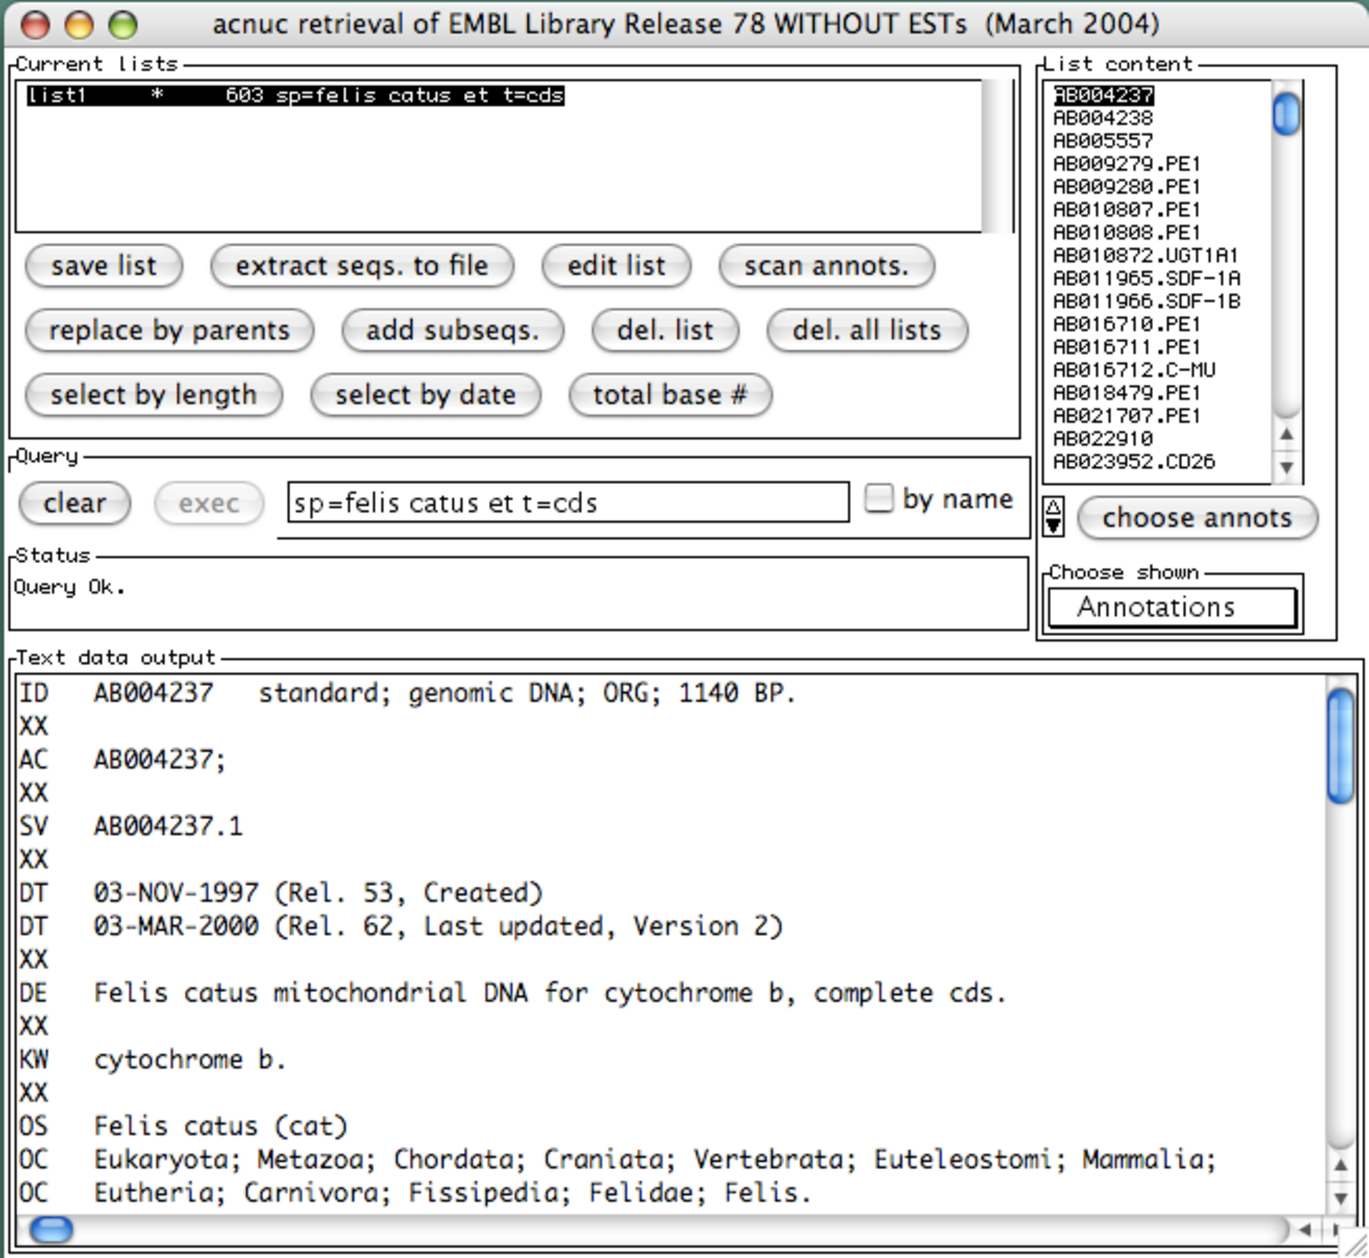
\includegraphics[width=\textwidth]{../figs/query_win_screenshot}
\caption{Screenshot of query\_win}
\label{queryw}
\end{minipage}
}
\end{figure}


Note:
The \textit{local} version of \textbf{query} is distributed with the ACNUC management  tools,
 thus it is already available in your ./ACNUC\_HOME/ACNUC\_SOFT/tools/ directory.
Before using it you need to set two environment  variables, \textit{acnuc} and \textit{gcganuc} :
\begin{verbatim}
setenv acnuc MYDATABASE/index
setenv gcgacnuc MYDATABASE/flat_files 
\end{verbatim}

where MYDATABASE is the path to the database you want to query ( for example: ./ACNUC\_HOME/ACNUC\_DB/demoacnuc/
 or ./ACNUC\_HOME/ACNUC\_DB/mydb/)
  
 




%%%%%%%%%%%%%%%%%%%%%%%%%%%%%%%%%%%%%%%%%%%%%%%%%%%%%
\section{Technical description of the racnucd daemon}
%%%%%%%%%%%%%%%%%%%%%%%%%%%%%%%%%%%%%%%%%%%%%%%%%%%%%
Technical information about the acnuc socket server is available at this url:
\url{http://pbil.univ-lyon1.fr/databases/acnuc/racnucd.html}.

%%%%%%%%%%%%%%%%%%%%%%%%%%%%%%%%%%%%%
\section{ACNUC remote access protocol}
%%%%%%%%%%%%%%%%%%%%%%%%%%%%%%%%%%%%%
Description of the socket communication protocol with acnuc is availble at this url:
\url{http://pbil.univ-lyon1.fr/databases/acnuc/remote_acnuc.html}




\section{Citation} 
%%%%%%%%%%%%%

You can use a citation along these lines:

\vspace{0.2cm}

\noindent\fbox{\begin{minipage}{\textwidth}
\noindent Sequences from [\textit{cite your source of data}] were structured under the 
ACNUC model \cite{acnuc1985}, hosted [at \textit{give your URL if
public}] by an ACNUC server \cite{acnuc2007} and analyzed with 
the \seqinr{} client \cite{seqinr} under the \Rlogo{} statistical environment \cite{RfromR}.
\end{minipage}}

\vspace{0.2cm}

For \LaTeX{} users, these references are available in the \texttt{book.bib} file that ships
with \seqinr{} in the \texttt{seqinr/doc/src/config/} folder. To locate this file on your
computer try:

\begin{Schunk}
\begin{Sinput}
 (seqinrloc <- normalizePath(.path.package("seqinr")))
\end{Sinput}
\begin{Soutput}
[1] "/Users/lobry/seqinr/pkg.Rcheck/seqinr"
\end{Soutput}
\begin{Sinput}
 setwd(seqinrloc)
 dir()
\end{Sinput}
\begin{Soutput}
 [1] "CITATION"    "CONTENTS"    "DESCRIPTION" "INDEX"       "Meta"       
 [6] "R"           "R-ex"        "data"        "doc"         "help"       
[11] "html"        "latex"       "libs"        "man"         "sequences"  
\end{Soutput}
\begin{Sinput}
 setwd("./doc/src/config")
 dir()
\end{Sinput}
\begin{Soutput}
[1] "atxy.sty"        "book.bib"        "commonrnw.rnw"   "commontex.tex"  
[5] "sessionInfo.rnw"
\end{Soutput}
\begin{Sinput}
 cat(readLines("book.bib", n = 5), sep = "\n")
\end{Sinput}
\begin{Soutput}
@incollection{seqinr,
    author = {Charif, D. and Lobry, J.R.},
    title = {Seqin{R} 1.0-2: a contributed package to the {R} project for statistical computing devoted to biological sequences retrieval and analysis.},
    booktitle = {Structural approaches to sequence evolution: Molecules, networks, populations},
    year = {2007},
\end{Soutput}
\end{Schunk}

%
% For Sweave users, go back home:
%


\section*{Session Informations}

This part was compiled under the following \Rlogo{}~environment:

\begin{itemize}
  \item R version 2.8.0 (2008-10-20), \verb|i386-apple-darwin8.8.2|
  \item Locale: \verb|C|
  \item Base packages: base, datasets, grDevices, graphics, methods,
    stats, utils
  \item Other packages: MASS~7.2-44, ade4~1.4-9, ape~2.2-2,
    nlme~3.1-89, quadprog~1.4-11, seqinr~2.0-0, tseries~0.10-16,
    xtable~1.5-4, zoo~1.5-4
  \item Loaded via a namespace (and not attached): grid~2.8.0,
    lattice~0.17-15, tools~2.8.0
\end{itemize}
There were two compilation steps:

\begin{itemize}
  \item \Rlogo{} compilation time was: Sun Oct 26 18:13:58 2008
  \item \LaTeX{} compilation time was: \today
\end{itemize}

% END - DO NOT REMOVE THIS LINE

%%%%%%%%%%%%  BIBLIOGRAPHY %%%%%%%%%%%%%%%%%
\clearpage
\addcontentsline{toc}{section}{References}
\bibliographystyle{plain}
\bibliography{../config/book}
\end{document}
